\documentclass[journal,12pt,twocolumn]{IEEEtran}

\usepackage{setspace}
\usepackage{gensymb}
\singlespacing
\usepackage[cmex10]{amsmath}

\usepackage{amsthm}

\usepackage{mathrsfs}
\usepackage{txfonts}
\usepackage{stfloats}
\usepackage{bm}
\usepackage{cite}
\usepackage{cases}
\usepackage{subfig}

\usepackage{longtable}
\usepackage{multirow}

\usepackage{enumitem}
\usepackage{mathtools}
\usepackage{steinmetz}
\usepackage{tikz}
\usepackage{circuitikz}
\usepackage{verbatim}
\usepackage{tfrupee}
\usepackage[breaklinks=true]{hyperref}
\usepackage{graphicx}
\usepackage{tkz-euclide}

\usetikzlibrary{calc,math}
\usepackage{listings}
    \usepackage{color}                                            %%
    \usepackage{array}                                            %%
    \usepackage{longtable}                                        %%
    \usepackage{calc}                                             %%
    \usepackage{multirow}                                         %%
    \usepackage{hhline}                                           %%
    \usepackage{ifthen}                                           %%
    \usepackage{lscape}     
\usepackage{multicol}
\usepackage{chngcntr}

\DeclareMathOperator*{\Res}{Res}

\renewcommand\thesection{\arabic{section}}
\renewcommand\thesubsection{\thesection.\arabic{subsection}}
\renewcommand\thesubsubsection{\thesubsection.\arabic{subsubsection}}

\renewcommand\thesectiondis{\arabic{section}}
\renewcommand\thesubsectiondis{\thesectiondis.\arabic{subsection}}
\renewcommand\thesubsubsectiondis{\thesubsectiondis.\arabic{subsubsection}}


\hyphenation{op-tical net-works semi-conduc-tor}
\def\inputGnumericTable{}                                 %%

\newcommand{\permcomb}[4][0mu]{{{}^{#3}\mkern#1#2_{#4}}}
\newcommand{\perm}[1][-3mu]{\permcomb[#1]{P}}
\newcommand*{\comb}[1][-1mu]{\permcomb[#1]{C}}

\lstset{
%language=C,
frame=single, 
breaklines=true,
columns=fullflexible
}
\begin{document}

\newcommand{\BEQA}{\begin{eqnarray}}
\newcommand{\EEQA}{\end{eqnarray}}
\newcommand{\define}{\stackrel{\triangle}{=}}
\bibliographystyle{IEEEtran}
\raggedbottom
\setlength{\parindent}{0pt}
\providecommand{\mbf}{\mathbf}
\providecommand{\pr}[1]{\ensuremath{\Pr\left(#1\right)}}
\providecommand{\qfunc}[1]{\ensuremath{Q\left(#1\right)}}
\providecommand{\sbrak}[1]{\ensuremath{{}\left[#1\right]}}
\providecommand{\lsbrak}[1]{\ensuremath{{}\left[#1\right.}}
\providecommand{\rsbrak}[1]{\ensuremath{{}\left.#1\right]}}
\providecommand{\brak}[1]{\ensuremath{\left(#1\right)}}
\providecommand{\lbrak}[1]{\ensuremath{\left(#1\right.}}
\providecommand{\rbrak}[1]{\ensuremath{\left.#1\right)}}
\providecommand{\cbrak}[1]{\ensuremath{\left\{#1\right\}}}
\providecommand{\lcbrak}[1]{\ensuremath{\left\{#1\right.}}
\providecommand{\rcbrak}[1]{\ensuremath{\left.#1\right\}}}
\theoremstyle{remark}
\newtheorem{rem}{Remark}
\newcommand{\sgn}{\mathop{\mathrm{sgn}}}
\providecommand{\abs}[1]{\vert#1\vert}
\providecommand{\res}[1]{\Res\displaylimits_{#1}} 
\providecommand{\norm}[1]{\lVert#1\rVert}
%\providecommand{\norm}[1]{\lVert#1\rVert}
\providecommand{\mtx}[1]{\mathbf{#1}}
\providecommand{\mean}[1]{E[ #1 ]}
\providecommand{\fourier}{\overset{\mathcal{F}}{ \rightleftharpoons}}
%\providecommand{\hilbert}{\overset{\mathcal{H}}{ \rightleftharpoons}}
\providecommand{\system}{\overset{\mathcal{H}}{ \longleftrightarrow}}
	%\newcommand{\solution}[2]{\textbf{Solution:}{#1}}
\newcommand{\solution}{\noindent \textbf{Solution: }}
\newcommand{\cosec}{\,\text{cosec}\,}
\providecommand{\dec}[2]{\ensuremath{\overset{#1}{\underset{#2}{\gtrless}}}}
\newcommand{\myvec}[1]{\ensuremath{\begin{pmatrix}#1\end{pmatrix}}}
\newcommand{\mydet}[1]{\ensuremath{\begin{vmatrix}#1\end{vmatrix}}}
\numberwithin{equation}{subsection}
\makeatletter
\@addtoreset{figure}{problem}
\makeatother
\let\StandardTheFigure\thefigure
\let\vec\mathbf
\renewcommand{\thefigure}{\theproblem}
\def\putbox#1#2#3{\makebox[0in][l]{\makebox[#1][l]{}\raisebox{\baselineskip}[0in][0in]{\raisebox{#2}[0in][0in]{#3}}}}
     \def\rightbox#1{\makebox[0in][r]{#1}}
     \def\centbox#1{\makebox[0in]{#1}}
     \def\topbox#1{\raisebox{-\baselineskip}[0in][0in]{#1}}
     \def\midbox#1{\raisebox{-0.5\baselineskip}[0in][0in]{#1}}
\vspace{3cm}
\title{AI1103-Assignment 7}
\author{Name : Aayush Patel, Roll No.: CS20BTECH11001}
\maketitle
\newpage
\bigskip
\renewcommand{\thefigure}{\theenumi}
\renewcommand{\thetable}{\theenumi}
Python codes : 
\begin{lstlisting}
https://github.com/Aayush-2492/Assignments/tree/main/Assignment7/code
\end{lstlisting}
%
Latex codes : 
%
\begin{lstlisting}
https://github.com/Aayush-2492/Assignments/tree/main/Assignment7
\end{lstlisting}
\section*{CSIR UGC NET EXAM (June 2013), Q.42}
Consider a parallel system with two components. The lifetimes of the two components are independent and identically distributed random variables each following an exponential distribution with mean 1. The expected lifetime of the system is:
\begin{enumerate}[label=\Alph*)]
    \item $1$\\[0.5pt]
    \item $\dfrac{1}{2}$\\
    \item $\dfrac{3}{2}$\\
    \item $2$
\end{enumerate}
\section*{Solution}
Consider two random variables X and Y which represent the lifetime of the two components namely A and B.
\begin{equation}
    X \sim Exp(\lambda_X)
\end{equation}
\begin{equation}
    Y \sim Exp(\lambda_Y)
\end{equation}
\begin{figure}[h]
    \centering
    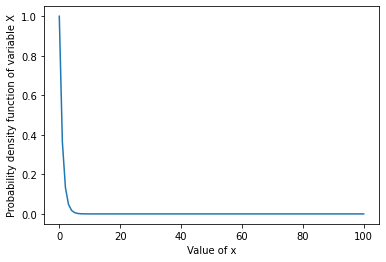
\includegraphics[width=\columnwidth]{figure2.png}
    \caption{P.D.F. of X }
    \label{fig:fig_label}
\end{figure}
Let $f_X(x)$ denote the probability distribution function for random variable X.
\begin{align}
f_{X}(x)=
 \begin{cases} 
      \lambda_X  e^{-\lambda_X  x} & x \geq 0 \\
      0 & otherwise
 \end{cases}
\end{align}
Let $f_Y(y)$ denote the probability distribution function for random variable Y.
\begin{align}
f_{Y}(y)=
 \begin{cases} 
      \lambda_Y  e^{-\lambda_Y  y} & y \geq 0 \\
      0 & otherwise
 \end{cases}
 \end{align}
 Let $F_X(x)$ denote the cumulative distribution function for random variable X.
\begin{align}
F_{X}(x)=
 \begin{cases} 
      1-e^{-\lambda_X  x} & x \geq 0 \\
      0 & otherwise
 \end{cases}
\end{align}
Let $F_Y(y)$ denote the cumulative distribution function for random variable Y.
\begin{align}
F_{Y}(y)=
 \begin{cases} 
      1-e^{-\lambda_Y  y} & y \geq 0 \\
      0 & otherwise
 \end{cases}
 \end{align}
\begin{equation}\label{meanx}
    E(X)=\dfrac{1}{\lambda_X}
\end{equation}
\begin{equation}\label{meany}
    E(Y)=\dfrac{1}{\lambda_Y}
\end{equation}
From \ref{meanx} and \ref{meany},
\begin{equation}\label{lambda}
    \lambda_X = \lambda_Y = 1
\end{equation}
\begin{figure}[h]
    \centering
    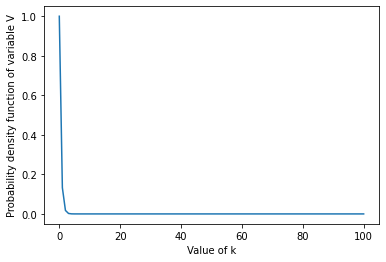
\includegraphics[width=\columnwidth]{figure.png}
    \caption{Parallel system}
    \label{fig:fig_label}
\end{figure}
Let Z be a random variable such that $Z=max(X,Y)$
\begin{align}
    P(Z\leq z) &= P(max(X,Y) \leq z)
    \\
    &=P(X\leq z,Y\leq z)
    \\
    &=P(X\leq z) P(Y\leq z)
    \\
    &=(F_X(z)-F_X(0)) (F_Y(z)-F_Y(0))
    \\
    &=1-e^{-(\lambda_X) z}-e^{-(\lambda_Y) z}+e^{-(\lambda_X+\lambda_Y) z}
\end{align}
$P(Z\leq z)$ denotes the probability that the system dies in the first $z$ seconds.\\
\begin{align}
    Expectation &= \int_{0}^{\infty}z \,d(P(Z\leq z))
    \\
\nonumber    &=\int_{0}^{\infty}z(\lambda_Xe^{-(\lambda_X) z}+\lambda_Ye^{-(\lambda_Y) z}\\
&-(\lambda_X+\lambda_Y)e^{-(\lambda_X+\lambda_Y) z}) \,dz
    \\
    &= \dfrac{1}{\lambda_X}+\dfrac{1}{\lambda_Y}-\dfrac{1}{\lambda_X+\lambda_Y}
\end{align}
From \ref{lambda}, 
\begin{equation}
    Expectation=\dfrac{3}{2}
\end{equation}
Therefore, option C correct.
\\
\end{document}
